% !TeX program = xelatex ?me -synctex=0 -interaction=nonstopmode -aux-directory=../tex_aux -output-directory=./release
% !TeX program = xelatex

\documentclass[12pt]{book}

\usepackage{lineno,changepage,lipsum}
\usepackage[colorlinks=true,urlcolor=blue]{hyperref}
\usepackage{fontspec}
\usepackage{xeCJK}
\usepackage{tabularx}
\usepackage{graphicx}
\setCJKfamilyfont{chanto}{AozoraMinchoRegular.ttf}%
\setCJKfamilyfont{tegaki}{Mushin.otf}%
\usepackage[CJK,overlap]{ruby}
\usepackage{hhline}
\usepackage{multirow,array,amssymb}
\usepackage[croatian]{babel}
\usepackage{soul}
\usepackage[usenames, dvipsnames]{color}
\usepackage{wrapfig,booktabs}
\usepackage{calc}
\renewcommand{\rubysep}{0.1ex}
\renewcommand{\rubysize}{0.75}
\usepackage[margin=50pt]{geometry}
\usepackage{hyperref}
\modulolinenumbers[2]

\date{\today}

\usepackage{fancyhdr}
\pagestyle{fancy}
\fancyhf{}
\fancyhead[LE,RO]{\thepage}
\makeatletter
\fancyhead[RE,LO]{\the\year 誠}
\makeatother

\usepackage{pifont}
\newcommand{\cmark}{\ding{51}}%
\newcommand{\xmark}{\ding{55}}%

\newcommand{\dosl}{{\normalfont dosl. }}%
\newcommand{\rem}[1]{{\normalfont #1 }}%

\definecolor{faded}{RGB}{100, 100, 100}

\renewcommand{\arraystretch}{1.2}

%\ruby{}{}
%$($\href{URL}{text}$)$

\newcommand{\furigana}[2]{\ruby{#1}{#2}}
\newcommand{\tegaki}[1]{
	\CJKfamily{tegaki}\CJKnospace
	#1
	\CJKfamily{chanto}\CJKnospace
}

\newcommand{\dai}[1]{
	\vspace{20pt}
	\large
	\noindent\textbf{#1}
	\normalsize
	\vspace{20pt}
}

\newcommand{\fukudai}[1]{
	\vspace{10pt}
	\noindent\textbf{#1}
	\vspace{10pt}
}

\newenvironment{bunshou}{
	\vspace{10pt}
	\begin{adjustwidth}{1cm}{3cm}
	\begin{linenumbers}
}{
	\end{linenumbers}
	\end{adjustwidth}
}

\newenvironment{reibun}[1][]{
	\vspace{10pt}
	#1
	
	\begin{tabular}{l l}
}{
	\end{tabular}
	\vspace{10pt}
}
\newcommand{\rei}[2]{
	#1&\textit{#2}\\
}
\newcommand{\reinagai}[2]{
	\multicolumn{2}{l}{#1}\\
	\multicolumn{2}{l}{\hspace{10pt}\textit{#2}}\\
}

\newenvironment{mondai}[1]{
	\vspace{10pt}
	\noindent #1
	
	\begin{enumerate}
		\itemsep-5pt
	}{
	\end{enumerate}
}

\newenvironment{hyou}{
	\begin{itemize}
		\itemsep-5pt
	}{
	\end{itemize}
	\vspace{10pt}
}

\newcommand{\juuyou}[2][20pt]{
	\vspace{5pt}
		\noindent\hspace{#1}\parbox[c]{\textwidth-#1-#1}{\centering\textit{#2}}
	\vspace{5pt}
}

\newcommand{\ten}{
	\vspace{5pt}
	\noindent\hspace{-10pt}$\bullet$
}

\setcounter{tocdepth}{0}
\newcommand{\fakesection}[1]{%
	\par\refstepcounter{chapter}% Increase section counter
	\sectionmark{#1}% Add section mark (header)
	\addcontentsline{toc}{chapter}{\protect\numberline{}#1\xleaders\hbox{.}\hfill\kern0pt}
	% Add more content here, if needed.
}

\CJKfamily{chanto}\CJKnospace

\frenchspacing

\hypersetup{
	colorlinks = true,
	linkcolor = {black},
}
\usepackage{tikz}
\title{Skripta\\
\large za srednje radionice japanskog\\
Makoto}
\author{Katja Kržišnik, Kristijan Čavić, Tomislav Mamić}

\begin{document}

{\let\cleardoublepage\clearpage
\maketitle
\tableofcontents}
\newpage
\fakesection{023: Opisna rečenica}

	\dai{Opisna rečenica}
	
	\fukudai{Teorija - opis u japanskom}
	
	Dosad smo za opisivanje imenica, izuzev nekih primjera koje smo smatrali težima, koristili samo pridjeve. Naučili smo da pridjevi dolaze uglavnom u dvije vrste koje smo nazvali い i な pridjevima\footnotemark[1]. Međutim, japanski pridjevi za razliku od hrvatskih mogu nositi informacije o vremenu i negaciji, što nam je kompliciralo prijevod. Pogledajmo točno \textit{kako} se prijevod mijenja:
	
	\begin{reibun}
		\rei{くろい\furigana{猫}{ねこ}}{crna mačka}
		\rei{くろくない猫}{mačka koja nije crna}
	\end{reibun}
	
	Iako se u japanskom struktura rečenice nije značajnije promijenila, u hrvatskom smo pridjev morali zamijeniti cijelom zavisnom rečenicom \textit{koja nije crna} da bismo dodali negaciju. Međutim, pogledamo li pobliže くろくない, možemo uočiti da se radi o dva dijela koje smo već prije viđali, a koje znamo koristiti i odvojeno - くろく (prilog od くろい, \textit{crno}) i ない (negacija glagola ある, \textit{biti}). Možemo reći da je くろくない zapravo zavisna rečenica koja se sastoji od negiranog glagola ある i priloga くろく koji taj glagol opisuje.
	
	Ovakvo opisivanje predikatima jedan je od temeljnih mehanizama za građenje rečenica u japanskom jeziku.
	
	\footnotetext[1]{U jap. gramatici ove se vrste zovu 形容詞 (けい.よう.し) i 形容動詞 (けい.よう.どう.し).}
	
	\fukudai{Teorija - predikatni i opisni oblik}
	
	U prošlosti jezika, sve riječi koje su mogle poslužiti kao predikat imale su dva različita oblika - predikatni i opisni\footnotemark[2]. Kad bi služile kao predikat glavne rečenice, dolazile bi u predikatnom obliku, a kad bi bile predikat zavisne rečenice koja opisuje neku imenicu, koristio se opisni oblik. Pogledajmo primjere:

	\footnotetext[2]{U jap. gramatici 終止形 (しゅう.し.けい) i 連体形 (れん.たい.けい).}
	
	\begin{reibun}
		\rei{あかい くるま}{crveni auto \normalfont{(opis)}}
		\rei{くるまは あかい。}{Auto je crven. \normalfont{(predikat)}}
	\end{reibun}
	
	Nekad davno, pridjevi u ovim rečenicama razlikovali bi se po obliku (あかき i あかし), no u modernom jeziku い pridjevi su izgubili ove razlike. Na sličan način razlike su izgubili i glagoli pa su im danas oba oblika ista:
	
	\begin{reibun}
		\rei{りんごを 食べた。}{Pojeo sam jabuku. \normalfont{(predikat)}}
		\rei{食べた りんご}{jabuka koju sam pojeo \normalfont{(opis)}}
	\end{reibun}
	
	Jedina nama bitna skupina riječi u kojoj su se razlike zadržale do danas jesu な i の pridjevi koji u predikatnom obliku dolaze u kombinaciji sa spojnim glagolom:
	
	\begin{reibun}
		\rei{びょうきの人}{bolestan čovjek \normalfont{(opis)}}
		\rei{あの人は びょうきだ。}{Onaj čovjek je bolestan. \normalfont{(predikat)}}
		\rei{げんきな人}{zdrav / veseo čovjek \normalfont{(opis)}}
		\rei{あの人は げんきだ。}{Onaj čovjek je zdrav / veseo. \normalfont{(predikat)}}
	\end{reibun}
	
	\fukudai{Teorija - strogo opisne riječi}
	
	Osim dosad spomenutih opisa, u japanskom jeziku postoji još jedna kategorija opisnih riječi za čiji naziv u hrvatskom jeziku nemamo dobar prijevod pa ćemo ih zvati 連体詞 (れん.たい.し) kao u jap. gramatici. Neke od ovih riječi već smo koristili (npr. この, その, あの), a posebne su po tome što se pojavljuju isključivo kao opis imenice i što su nepromjenjive. Najčešći zbunjujući primjeri su:
	
	\begin{reibun}
		\rei{大きな いえ}{velika kuća \cmark}
		\rei{いえは 大きだ。}{Kuća je velika. \xmark~\normalfont{(mora biti 大きい)}}
		\rei{小さな 花}{mali cvijet}
		\rei{花は 小さだ。}{Cvijet je malen. \xmark~\normalfont{(mora biti 小さい)}}
	\end{reibun}

	Iako tako izgledaju, 大きな i 小さな \textbf{nisu} な pridjevi već opisne riječi. Ovakve opisne riječi vrlo su često nastale kao okamenjeni ili malo promijenjeni oblici drugih riječi pa ih je lako zamijeniti za druge vrste i krivo upotrijebiti, no na našu sreću, nema ih puno\footnotemark[3].
	
	\footnotetext[3]{Za istraživanje potražite "\#adj-pn" na jisho.org!}
	
	\fukudai{Tvorba opisnog oblika}
	
	Zahvaljujući promjenama u modernom jeziku, tablica u nastavku postala je veoma jednostavna. Komplikacije dolaze od imenica i な pridjeva čiji predikatni oblik stvaramo pomoću spojnog glagola だ. Naime gramatički gledano, opisni oblik tog glagola trebao bi uvijek biti な, ali u praksi to nije tako i imenice gotovo uvijek opisuju druge imenice česticom の\footnotemark[4].
	
	\footnotetext[4]{Uz imenice se な pojavljuje iznimno kad opisuju imenicu の(もの) i veznike nastale od iste - ので i のに.}
	
	\begin{table}[h]
		\centering
		\begin{tabular}{l c c}\toprule[2pt]
			vrsta predikata & predikatni oblik & opisni oblik\\
			\midrule
			imenica & \textasciitilde だ & \textasciitilde の\\
			な pridjev & \textasciitilde だ & \textasciitilde な\\
			い pridjev & \multicolumn{2}{c}{nema razlike}\\
			glagol & \multicolumn{2}{c}{nema razlike}\\
			\bottomrule[2pt]
		\end{tabular}
	\end{table}

	\fukudai{Tvorba i značenje opisne rečenice}
	
	Rečenica postaje opisna kad njezin predikat prebacimo u opisni oblik (što uglavnom znači da mu ne moramo napraviti ništa!) i umetnemo je u drugu rečenicu kao opis nekoj opisivoj riječi ili izrazu. Pri tome gotovo uvijek opisujemo riječ koju bismo morali umetnuti u zavisnu rečenicu da bi postala samostalna. Pogledajmo primjere:
	
	\begin{reibun}
		\reinagai{たけしくん\underline{は} りんごを食べた。$\rightarrow$たけしくん\underline{が}食べた りんご}{Takeši je pojeo jabuku. $\rightarrow$ jabuka koju je Takeši pojeo}
		\reinagai{きのう、田中さんは猫を見た。$\rightarrow$きのう猫を見た田中さん}{Tanaka je jučer vidio mačku. $\rightarrow$ Tanaka koji je jučer vidio mačku}
		\reinagai{おみせでコップを かった。$\rightarrow$コップを かった おみせ}{U dućanu sam kupio šalicu. $\rightarrow$ dućan u kojem sam kupio šalicu}
	\end{reibun}

	U primjerima iznad događa se par zanimljivih stvari koje ćemo u nastavku pobliže proučiti i objasniti.
	
	\vspace{5pt}
	\textbf{Subjekt} u opisnim rečenicama nikad nije tema. Opisne rečenice dodaju informacije o jednoj riječi u nadređenoj rečenici, a temu od nje preuzimaju. Pokušamo li smisliti protuprimjere, vidjet ćemo da takvo nešto ne funkcionira po smislu. U pravilu će subjekt dobiti česticu が ili の.
	
	Ova upotreba čestice の za označavanje subjekta u zavisnim rečenicama je česta i u početku može biti zbunjujuća, no prepoznat ćemo je po tome što, za razliku od slučaja gdje izriče posjedovanje ili opis, ovdje ne spaja dvije imenice već imenicu i predikat. Tako je prvi primjer iznad mogao glasiti i たけしくん\underline{の}食べた りんご bez razlike u značenju.
	
	\vspace{5pt}
	\textbf{Čestice} uz imenicu koju vadimo iz jednostavne rečenice mogu se razlikovati. Nakon što smo imenicu tako izvadili ispred, dobili smo komad rečenice\footnotemark[5] kojem je desni kraj imenica. Na tu ćemo imenicu dodati česticu koja nam treba da je smjestimo na željeno mjesto u glavnoj rečenici.
	
	\footnotetext[5]{Ili stručnije \textit{sintagma}.}
	
	Učinivši to, izbrisali smo informaciju o tome kako se opisana imenica uklapa u pridruženu joj opisnu rečenicu! Ovdje se japanski jezik oslanja na zdrav razum i govornikovu sposobnost da iz konteksta zaključi koji je njihov međusobni odnos. Usporedimo sljedeće primjere s onima iznad:
	
	\begin{reibun}
		\rei{りんごを食べた たけしくん}{Takeši koji je pojeo jabuku}
		\rei{田中さんが きのう見た猫}{mačka koju je Tanaka jučer vidio}
		\rei{おみせで かったコップ}{šalica koju sam kupio u dućanu}
		\reinagai{きのう はなした人}{čovjek o kojem sam (ti) jučer pričao \cmark čovjek koji je jučer pričao \cmark}
	\end{reibun}

	Uočavamo da je sadržaj rečenica isti, no ovaj put smo izvukli druge imenice. Njihovo mjesto u opisnoj rečenici pretpostavit ćemo prema tome koja u njoj informacija nedostaje, što za prva tri primjera nije preteško. Međutim, u trećem primjeru 人 može pričati, ali može biti i tema razgovora pa se moramo osloniti na kontekst da odaberemo ispravno tumačenje.
	
	\fukudai{Vježba}
	
	\begin{mondai}{Prevedite rečenice u nastavku.}
		\item 猫が わたしの にわで あそんでいる。
		\item 花子さんの いもうとが猫を見た。
		\item いつも猫と いっしょに いる。
		\item 猫に えさを あげた。 (えさ - \textit{hrana za životinje})
		\item かわいくて 小さい 猫だ。
		\item 猫が木に のぼった。 (のぼる - \textit{popeti se})
	\end{mondai}

	\noindent
	Preoblikujte prethodne rečenice u sintagme koje opisuju 猫.
	
	\vspace{5pt}\noindent
	Spojite proizvoljno parove rečenica tako da jednu rečenicu odaberete kao glavnu i onda u njoj 猫 opišete neko-m drugom. Hehe. He.

\newpage
\fakesection{024: Vremenske imenice}


\newcommand{\en}[1]{
	\begin{tikzpicture}[baseline=(C.base)]
	\node[draw,circle,inner sep=1pt](C){#1};
	\end{tikzpicture}
}

	\dai{Vremenske imenice}
	
	\fukudai{Teorija - priložne imenice}
	
	Ovu smo temu okrznuli na početnim radionicama kad smo učili o priložnim oznakama vremena. Tada smo rekli da u japanskom jeziku postoje imenice koje imaju gramatičku funkciju - koje određuju odnos između svog opisa i ostatka rečenice, i tu smo stali. Sada, znajući ponešto o opisnim rečenicama, možemo u detalje proučiti ovaj vrlo važan gramatički mehanizam. Uzmimo za primjer neke česte vremenske imenice:
	
	\begin{reibun}
		\rei{とき}{vrijeme}
		\rei{ころ}{vrijeme, period, razdoblje}
		\rei{しゅんかん}{trenutak}
	\end{reibun}

	\noindent
	Nabrojane imenice imaju konkretno značenje - rečenici mogu dodati sadržaj:
	
	\begin{reibun}
		\rei{その ときが 来た。}{Došlo je to vrijeme.}
	\end{reibun}

	\noindent
	Vrlo je često neprirodno prevoditi ili uopće razmatrati konkretno značenje priložnih imenica:
	
	\begin{reibun}
		\reinagai{猫を見た ときの 花子ちゃんの えがおは わすれません。}{Neću zaboraviti osmjeh koji je Hanako imala na licu kad je vidjela mačku.}
		\reinagai{日本に すんでいた ころ、まいにち ラーメンを 食べていた。}{Kad sam živio u Japanu, svaki dan sam jeo r\={a}men.}
	\end{reibun}

	\noindent
	Uočimo kako u rečenicama iznad nismo preveli ni とき ni ころ, već smo njihove opise u hrvatskom preveli kao zavisne rečenice koje opisuju vrijeme glavne. Ovo je bitna osobina svih priložnih imenica.
	
	\fukudai{Opisivanje \textit{kad} se nešto dogodilo}
	
	Već znamo reći da se nešto dogodilo \textit{jučer} ili \textit{prošle godine}. Koristeći vremenske imenice možemo sastaviti složene rečenice s vrlo bogatim priložnim oznakama vremena. Uz dvije ranije spomenute rečenice, pogledajmo primjere:
	
	\begin{reibun}
		\reinagai{こどもの ころ、川の そばで あそんでいた。}{Kao dijete sam se često igrao u blizini rijeke.}
		\reinagai{みちを わたる とき、くるまに きを つけてください。}{Kad prelaziš cestu, pazi na aute.}
		\reinagai{\parbox{480pt}{猫に 気が ついた\footnotemark[1] しゅんかん、たけしは へんな こえを 出しました。}}{\parbox{480pt}{U trenu kad je spazio mačku, Takeši je ispustio čudan zvuk.}}
		\reinagai{かれに であった あの日は いまも よく おぼえている。}{I sad se dobro sjećam onog dana kad sam ga upoznao.}
	\end{reibun}

	\footnotetext[1]{Izraz 気が(<nešto>に)つく koristi se sa značenjem \textit{primijetiti} <nešto>.}

	Uočimo kako je prijevod ovih priložnih oznaka vremena vrlo proizvoljan (npr. \textit{kao dijete sam} umjesto \textit{kad sam bio dijete}) - bitno je prenijeti značenje u duhu jezika, a ne gramatičku strukturu.

	\pagebreak
	\fukudai{Opisivanje intervala u kojem se nešto dogodilo}
	
	Koristeći imenice あいだ i うち (obje u rječniku imaju preko nekoliko različitih prijevoda) možemo izraziti značenje koje u hrvatskom postižemo riječju \textit{dok}:
	
	\begin{reibun}
		\reinagai{ともだちを まっている あいだ(に)、本を よんでいた。}{Dok sam čekao prijatelja, čitao sam knjigu.}
		\reinagai{ははが 食べている うちに、たけしくんは いえを でた。}{Dok je majka jela, Takeši je izišao iz kuće.}
		\reinagai{ちかい うちに\footnotemark[2] あらしが 来る。}{Uskoro dolazi oluja.}
	\end{reibun}

	U primjerima s glagolima iznad, zgodno je uočiti da predikati zavisnih rečenica izriču trenutno stanje (\textasciitilde ている) i da su u potvrdnom, neprošlom obliku. Imenice あいだ i うち u ovoj upotrebi \textbf{nikad nećemo opisivati} predikatom u prošlom vremenu. Negiramo li predikat, značenje se prigodno mijenja:
	
	\begin{reibun}
		\reinagai{ははが 見ていないうちに、たけしくんは いえを でた。}{Dok majka nije gledala, Takeši je izišao iz kuće.}
		\reinagai{先生が まだ 来ていない あいだに まどから きょうしつに はいった。}{Dok učitelj još nije došao, ušao sam u učionicu kroz prozor.}
	\end{reibun}

	\noindent
	Ukoliko negirani predikat ne izriče stanje, dobivamo nešto drugačiji smisao:
	
	\begin{reibun}
		\reinagai{先生が 来ない うちに まどから きょうしつに はいる。}{Ući ću u učionicu kroz prozor prije nego učitelj dođe.}
		\reinagai{花子ちゃんは さくらの花が ちらない うちに 日本に もどりたい。}{Hanako se želi vratiti u Japan prije nego trešnje ocvatu.}
	\end{reibun}

	\footnotetext[2]{Izraz ちかいうちに kao \textit{uskoro, ubrzo} je čest i koristan. Ovdje nije uobičajeno reći あいだ.}
	
	Gledajući brojeve na slici u nastavku, možemo im pridružiti sljedeće događaje:
	
	\begin{hyou}
		\item \en{1} さくらの花が さく
		\item \en{2} さくらの花が ちる
		\item \en{3} さくらの花が さいている うちに
		\item \en{4} さくらの花が ちらない うちに
	\end{hyou}
	
	\begin{figure}[h]
		\centering
		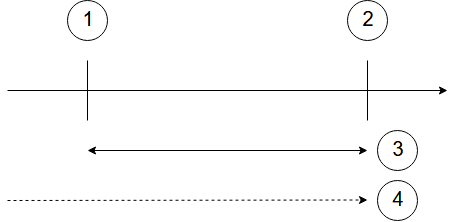
\includegraphics[width=200pt]{img/vrem_1}
		\caption{Trenuci na koje upućuju upotrebe \textasciitilde~うちに.}
	\end{figure}

	\fukudai{Vježba}
	
	\begin{mondai}{Prevedite na hrvatski:}
		\item きょねん 日本に 行った ときは さむかった。
		\item こどもの ころ、にんじんが きらいだった。
		\item ねずみを 見た しゅんかん、猫は 目を さました。\\(目を さます - izraz, \textit{probuditi se})
		\item こどもが ねている あいだは しずかに してください。\\(しずかに する - izraz, \textit{biti tiho})
		\item 花子ちゃんが いえに いない とき、猫は さびしく なる。\\(さびしい - \textit{usamljen})
		\item 花子ちゃんが いえに いない あいだに 猫は まくらの うえで ねていた。\\(まくら - \textit{jastuk})
		\item ごはんが さめない うちに たべてください。\\(さめる - \textit{ohladiti se})
	\end{mondai}

	\begin{mondai}{Prevedite na japanski:}
		\item Sljedeći put kad odeš u Japan, kupi mi neki suvenir.\\korisno: こんど - \textit{sljedeći put}, おみやげ - \textit{suvenir}
		\item Kad sam bio dijete sam mrzio mrkve, ali sada ih volim.
		\item Čim je čuo Hanako, Takeši je ušao u kutiju.\\korisno: とたん - slično kao しゅんかん, ali se često prevodi kao \textit{čim}
		\item Dok se Takeši igrao, Hanako je napisala domaću zadaću.\\korisno: しゅくだい domaća zadaća
		\item Želim se vratiti kući prije nego počne kiša.
	\end{mondai}

\newpage
\fakesection{025: Priložne imenice I}

	\dai{Priložne imenice I}
	
	\fukudai{Teorija}
	
	Imenice koje ćemo proučiti u nastavku spadaju u vrlo specifičnu skupinu \textit{lažnih} ili \textit{formalnih} imenica\footnotemark[1]. Zovu se tako jer, iako ćemo ih pronaći u rječnicima, i iako će imati nerijetko mnogo raznih prijevoda, ove se imenice u praksi gotovo nikad ne koriste niti tumače kao takve - \textbf{imaju gramatičku funkciju}.
	
	\footnotetext[1]{jap. 形式名詞 - けい.しき.めい.し, dosl. \textit{formalne imenice}}
	
	\fukudai{ため - svrha, cilj, poticaj, uzrok}
	
	\noindent
	Ovu ćemo riječ naći uglavnom u jednoj od dvije upotrebe:
	
	\vspace{5pt}\noindent
	Kad označava (pozitivnu) svrhu rečenice, npr. こどものため - \textit{(ono što je dobro) za dijete}:
	
	\begin{reibun}
		\rei{こどもの ために がっこうを たてた。}{Za djecu su sagradili školu.}
		\rei{あなたの ために 言っています。}{Govorim to za tvoje dobro.}
	\end{reibun}

	\noindent\vspace{5pt}
	Isto značenje dobivamo i kad ため opišemo rečenicom:
	
	\begin{reibun}
		\reinagai{いい がっこうに 行くために 花子ちゃんは いっしょうけんめい\footnotemark[2] べんきょう した。}{Kako bi išla u dobru školu, Hanako je učila što je bolje mogla.}
		\reinagai{たけしくんは つよく なる ために まいにち しゅぎょう している。}{Takeši svaki dan trenira da bi postao jak.}
	\end{reibun}

	\footnotetext[2]{pril. izražava veliki trud subjekta u izvršenju radnje rečenice}
	
	\vspace{5pt}\noindent
	U raspoznavanju značenja uzroka u odnosu na prethodno objašnjenu upotrebu pomažu nam samo kontekst i značenje rečenica:
	
	\begin{reibun}
		\reinagai{あらしの ために しあいを えんきしました。}{Za oluju smo odgodili utakmicu. \xmark\ Zbog oluje smo odgodili utakmicu. \cmark}
	\end{reibun}

	\noindent
	Ovakva upotreba ため je vrlo formalna i u svakodnevnom se razgovoru ne pojavljuje, no često je možemo čuti u vijestima i ostalim oblicima službenog izvještavanja.
	
	\fukudai{はず - vlastito uvjerenje, pretpostavka, zaključak}
	
	Vrlo često dolazi u jednostavnom obliku <rečenica>はずだ / です, no to nije gramatičko pravilo i ima situacija gdje se koristi u složenijim rečenicama. Bitno za ovu riječ je da je uvijek iz perspektive govornika, a \textbf{ne nužno subjekta} rečenice.
	
	\begin{reibun}
		\rei{でんしゃは そろそろ つく はずです。}{Vlak bi trebao uskoro stići.}
		\rei{でんしゃは もう ついた はずです。}{Vlak je vjerojatno već stigao.}
		\rei{たけしくんが 私の りんごを 食べた はずだ。}{Sigurno mi je Takeši pojeo jabuku.}
	\end{reibun}

	\newpage\noindent
	U prethodnim rečenicama, uvjerenje govornika je trenutno važeće. Promotrimo što se dogodi sa značenjem ako glavnu rečenicu prebacimo u prošlost:
	
	\begin{reibun}
		\rei{でんしゃは そろそろ つく はずだった。}{Mislio sam da će vlak uskoro stići.}
		\rei{でんしゃは もう ついた はずだった。}{Mislio sam da je vlak već trebao stići.}
	\end{reibun}

	\noindent
	U prethodna dva primjera implicira se da je govornikovo uvjerenje promijenjeno ili poljuljano - na kraj bismo mogli dodati \textit{ali sada više tako ne mislim} ili \textit{ali nešto nije kako treba}.
	
	\vspace{5pt}\noindent
	Uz dosad pokazane upotrebe, vrlo je čest izraz \textasciitilde はずがない. Značenje tog izraza je nešto teže pogoditi iz osnovnog značenja riječi:
	
	\begin{reibun}
		\reinagai{でんしゃが もう ついた はずが ない。}{Nema šanse da je vlak već stigao.}
		\reinagai{花子ちゃんが たけしくんに すうがくを おしえる はずが ない。}{Nema šanse da će Hanako pokazati Takešiju matematiku.}
	\end{reibun}

	\noindent
	Uočimo da je u ovom slučaju simetrija s hrvatskim dosta zanimljiva - uspoređujući \textit{nema šanse} i はずが ない mogli bismo poistovjetiti hrv. \textit{šanse} i jap. はず.
	
	\fukudai{つもり - namjera}
	
	Opis koji pridružimo つもり izražava namjeru subjekta rečenice. Iako ima punu gramatičku slobodu imenice, つもり se zbog svog smisla pretežno pojavljuje u dvije situacije. Kad jednostavno želimo izreći nečiju namjeru, reći ćemo:
	
	\begin{reibun}
		\reinagai{来年、日本に行く つもり です。}{Sljedeće godine namjeravam ići u Japan.}
		\reinagai{たけしくんは花子ちゃんに すうがくを おそわる\footnotemark[3] つもり だ。}{Takeši namjerava naučiti matematiku od Hanako.}
	\end{reibun}

	\footnotetext[3]{Glagol おそわる (\textit{naučiti od}) je drugačija perspektiva na おしえる (\textit{podučiti})!}

	\noindent
	O namjeri možemo govoriti u prošlosti bez ikakvih iznenađenja:
	
	\begin{reibun}
		\reinagai{きょねん、日本に行く つもり だった。}{Prošle sam godine namjeravao ići u Japan.}
		\reinagai{たけしくんは わたしのケーキを食べる つもり でした。}{Takeši je namjeravao pojesti moju tortu.}
	\end{reibun}

	\noindent
	Međutim, kad želimo reći da nemamo neku namjeru, možemo to učiniti na dva suptilno različita načina:
	
	\begin{reibun}
		\reinagai{めいわくを かける\footnotemark[4] つもり \underline{じゃ} なかった。}{Nisam ti želio stvoriti probleme. \normalfont{(uzrokovali smo neželjene posljedice)}}
		\reinagai{さいしょから べんきょうする つもり\underline{は} なかった。}{Od početka nisam imao namjeru učiti. \normalfont{(dogodilo se upravo ono što smo planirali)}}
	\end{reibun}

	\footnotetext[4]{Izraz めいわくを かける je vrlo kulturološki važan - često se pojavljuje i korisno ga je zapamtiti.}

	\newpage\noindent
	Često želimo reći da je nešto učinjeno \textit{s nekom namjerom}. To ćemo učiniti koristeći česticu で kao u primjerima u nastavku:
	
	\begin{reibun}
		\reinagai{日本に行く つもりで おかねを ためています。}{Štedim s namjerom da odem u Japan.}
		\reinagai{たけしくんは わたしの ケーキを食べる つもりで いえに はいった。}{Takeši je ušao u kuću s namjerom da pojede moju tortu.}
	\end{reibun}

	\fukudai{Vježba}
	
	\begin{mondai}{Dodajte razloge na sljedeće rečenice tako da odgovaraju na pitanje \textit{zašto} ili \textit{za koga}.}
		\item アイスクリームを かいました。
		\item まいにち べんきょう している。
	\end{mondai}

	\begin{mondai}{Dovršite rečenice dijelom kojeg je uzrokovao već napisani dio.}
		\item じこが あった ため
		\item 日本に行くため
	\end{mondai}

	\begin{mondai}{Prevedite na japanski.}
		\item \textit{Vjerojatno će stati u vreću.}
		\item \textit{Nema šanse da stane u vreću.}
	\end{mondai}

	\begin{mondai}{Prevedite na hrvatski.}
		\item この猫を ふくろの中に いれる つもりだ。
		\item 猫を ふくろの中に いれて もんだいを おこす つもり じゃ なかった。
	\end{mondai}
\newpage
\fakesection{026: Nominalizacija}

	\dai{Nominalizacija}
	
	\fukudai{Uvod - formalne imenice}
	
	Jedan podskup imenica se u japanskom koristi na način da umjesto svog originalnog značenja mijenja značenje svoje opisne rečenice. Takve imenice vrlo rijetko shvaćamo doslovno, a prijevodi su im često nejasni i opširni. Iz perspektive hrvatskog jezika, prijevodi se mogu jako razlikovati ovisno o korištenoj imenici - gramatike se ovdje zamjetno razlikuju. (potražiti 形式名詞)
	
	\fukudai{Nominalizacija - の i こと}
	
	\juuyou[40pt]{Nominalizacija je gramatički mehanizam kojim se kao imenice ili imeničke sintagme koriste dijelovi govora koji to nisu.}
	
	Formalne imenice もの (skraćuje se u の) i こと služe za pretvaranje svog opisa u imenice. Iako im se upotreba djelomično preklapa, postoje situacije u kojima smijemo koristiti samo の ili samo こと. Pogledajmo niz primjera:
	
	\begin{reibun}
		\rei{アイスクリームが好きです。}{Volim sladoled.}
		\rei{アイスクリームを食べる。}{Jesti sladoled. (u kontekstu Pojest ću sladoled.)}
		\rei{アイスクリームを食べる人}{čovjek koji jede sladoled (sintagma)}
	\end{reibun}
	
	U prvom primjeru koristimo 好き kao dio imenskog predikata da opišemo アイスクリーム. To je moguće samo zato što je アイスクリーム imenica zdesna\footnotemark[1] pa može primiti česticu が. Drugi primjer je opet vrlo jednostavna rečenica koju u trećem primjeru koristimo kao opis imenice 人. U drugom primjeru, glagol たべる je predikatni oblik (završava nezavisnu rečenicu) dok je u trećem primjeru opisni oblik (završava opisnu rečenicu)\footnotemark[2]. Nominalizaciju možemo koristiti za značenja poput
	
	\begin{reibun}
		\rei{アイスクリームを食べる\underline{の}が好きです。}{Volim jesti sladoled.}
		\rei{日本語は\furigana{難}{むずか}しいと言う\underline{こと}が分かった。}{Shvatio sam da je japanski težak.}
		\rei{\furigana{彼}{かれ}が出る\underline{の}を\furigana{待}{ま}っています。}{Čekam da on iziđe.}
	\end{reibun}
	
	\fukudai{Razlike između の i こと}
	
	Gledajući značenja u rječniku, もの se definira kao konkretna stvar, nešto u fizičkom svijetu, dok je こと apstraktna stvar, ideja, događaj ili koncept. Međutim te definicije su u najboljem slučaju daleki podsjetnici na pravilno korištenje ovih riječi. Najbolja smjernica koja se da sročiti kao pravilo je to da se の većinom koristi za stvari koje su neposredne i/ili subjektivne, a こと za apstraktnije koncepte i situacije u kojima ne postoji direktna čvrsta veza između opisne rečenice i glavnog glagola.
	
	Slijede situacije u kojima nije dopušteno zamijeniti の i こと. Za sve situacije koje ovdje nisu pobrojane, dopušteno je (iako ne nužno uvijek prirodno) koristiti i jednu i drugu riječ.
	
	\footnotetext[1]{Po jednostavnom modelu <opis> imenica <gramatika>, \textit{imenica zdesna} označava frazu čija se desna strana s obzirom na gramatičke mogućnosti ponaša kao imenica.}
	
	\footnotetext[2]{U modernom jap. morfološka razlika između opisnog i predikatnog oblika je izgubljena za sve predikate osim imenskog s な/の pridjevima kojima je nepr. poz. predikatni oblik だ.}
	\newpage
	\fukudai{Isključivo こと}
	
	\ten Kad nominalizirani opis želimo iskoristiti kao dio imenskog predikata (uz だ/である):
	
	\begin{reibun}
		\rei{私の\furigana{趣味}{しゅみ}は\furigana{絵}{え}を\furigana{描}{か}く\underline{こと}です。}{Moj hobi je crtanje/slikanje.}
		\rei{私の\furigana{目的}{もく.てき}は\furigana{生}{い}きて\furigana{帰}{かえ}る\underline{こと}です。}{Moj cilj je vratiti se živ.}
	\end{reibun}
	
	Razlog zbog kojeg u ovim slučajevima obavezno koristimo こと je fiksni izraz za kraj rečenice u tonu objašnjavanja のです (više u nastavku). Naime, zamijenimo li こと u gornjim primjerima s の, značenje će se uvelike promijeniti i neće zvučati prirodno.
	
	\ten Kad je nominalizirani opis zapravo neupravni govor. To je gotovo uvijek slučaj s glagolima koji označavaju neki oblik misli ili komunikacije:
	
	\begin{reibun}
		\reinagai{田中さんが\furigana{間}{ま}に\furigana{合}{あ}わない\underline{こと}を\furigana{社長}{しゃちょう}に\furigana{伝}{つた}えます。}{Prenijet ću (to) da Tanaka neće stići na vrijeme šefu.}
	\end{reibun}
	
	\ten Kad je こと dio fiksnog izraza:
	
	\begin{reibun}
		\rei{そのクジラは空を飛ぶ\underline{ことも出来る}。}{Taj kit može čak i letjeti.}
		\rei{たけしくんは\furigana{転校}{てんこう}する\underline{ことになった}。}{Takeši će se prebaciti u drugu školu. (tako je ispalo)}
		\rei{たけしくんは学校を\furigana{辞}{や}める\underline{ことにした}。}{Takeši je odlučio odustati od škole. (svojevoljno)}
		\reinagai{たけしくんはクロアチアまで行った\underline{ことがある}のに、大阪に\furigana{一度}{いちど}も行った\underline{ことがない}。}{Iako je išao čak do Hrvatske, Takeši ni jednom nije bio u \={O}saki.}
		\rei{\furigana{毎日}{まいにち}一キロ走る\underline{ことにしています}。}{Trudim se svaki dan trčati jedan kilometar.}
	\end{reibun}
	
	\fukudai{Isključivo の}
	
	\ten S glagolima percepcije:
	
	\begin{reibun}
		\rei{\furigana{隣}{となり}の\furigana{家}{いえ}で\furigana{誰}{だれ}かが\furigana{叫}{さけ}ぶ\underline{の}が\furigana{聞}{き}こえた。}{Iz susjedne kuće se čulo kako netko viče.}
		\rei{たなかくんが\furigana{逃}{に}げようとしている\underline{の}を見た。}{Vidio sam kako Tanaka pokušava uteći.}
		\rei{\furigana{指先}{ゆびさき}で何かが\furigana{動}{うご}いている\underline{の}を\furigana{感}{かん}じた。}{Vrhovima prstiju sam osjetio kako se nešto miče.}
	\end{reibun}
	
	\newpage
	
	\ten Kao referenca na već spomenutu imenicu:
	
	\begin{reibun}
		\rei{A: どんな\furigana{車}{くるま}がほしいか。}{Kakav auto želiš?}
		\rei{B: \furigana{赤}{あか}い\underline{の}がいい。}{Neki crveni.}
	\end{reibun}
	
	U primjeru iznad, の se koristi umjesto ponavljanja imenice 車. Ovo je u govoru jako česta pojava, kao i u hrvatskom jeziku. Iako je mehanizam različit, nitko ne voli bespotrebno ponavljati već poznate informacije. U sljedećim primjerima ideja je ista, ali の zamjenjuje neku imenicu općenitijeg značenja (npr. とき、場所 itd.). O kojoj se točno imenici radi saznajemo u dijelu rečenice nakon の:
	
	\begin{reibun}
		\rei{たけしくんが生まれた\underline{の}は\furigana{東京}{とうきょう}です。}{Takeši se rodio u Tokiju.}
		\rei{たけしくんが生まれた\underline{の}は1991年です。}{Takeši se rodio '91.}
	\end{reibun}
	
	U japanskom jeziku je ovo zapravo oblik inverzije. Vrlo lako možemo preoblikovati rečenice iznad u očekivani poredak informacija:
	
	\begin{reibun}
		\rei{たけしくんは東京に生まれた。}{Takeši se rodio u Tokiju.}
		\rei{たけしくんは1991年に生まれた。}{Takeši se rodio '91.}
	\end{reibun}
	
	Zanimljivo, isti mehanizam možemo iskoristiti i za spoj から:
	
	\begin{reibun}
		\rei{たけしくんが行きたくなかった\underline{の}は\furigana{高}{たか}い\furigana{所}{ところ}が\furigana{怖}{こわ}いからだった。}{Takeši nije htio ići jer se boji visine.}
		\rei{たけしくんは高い所が怖いから行きたくなかった。}{Takeši nije htio ići jer se boji visine.}
	\end{reibun}

	Svrha ovakve inverzije je isticanje informacije kao vrlo važne. U pravilu, ono što se nalazi bliže kraju rečenice u japanskom, smatra se bitnijim sadržajem.
	
	\ten Kao dio fiksnog izraza za objašnjenje/uvjeravanje のだ:
	
	\begin{reibun}
		\rei{A: びしょ\furigana{濡}{ぬ}れじゃないか。}{Mokar si do kože! (wtf?)}
		\rei{B: \furigana{池}{いけ}に\furigana{落}{お}ちてしまった\underline{んだ}。}{Upao sam u jezerce. (objašnjenje)}
		\reinagai{池に落ちてしまった\underline{ので}びしょ濡れです。}{Mokar sam do kože jer sam upao u jezerce.}
	\end{reibun}
	
	Dobro je zapamtiti da spojni glagol u japanskom dolazi u kolokvijalnoj i pristojnoj inačici (だ,\linebreak です), kao i da je skraćivanje の u ん jako česta pojava, čak i u pristojnom govoru.
	
	Treći primjer iznad trebao bi nam biti otprije poznat kao spoj ので. Naime, upravo je ovo porijeklo tog spoja - zapravo se radi o て obliku spojnog glagola だ$\rightarrow$で.
\newpage
\fakesection{027: Usporedbe I}

	\dai{Usporedbe I}
	
	\fukudai{Uvod}
	
	Iako je u japanske pridjeve upakirano više informacija nego u hrvatskom jeziku, naši pridjevi obavljaju jednu funkciju koju japanski ne mogu - usporedbu. Oblici pridjeva za usporedbu zovu se \textit{komparativ} (npr. \textit{dobar} $\rightarrow$ \textit{bolji}) i superlativ (npr. \textit{dobar} $\rightarrow$ \textit{najbolji}). Uočimo kako za upotrebu komparativa trebamo dvije stvari koje ćemo usporediti: kažemo li da je nešto \textit{bolje}, prirodno je pitati se \textit{od čega}.
	
	\fukudai{Čestica より za usporedbu}
	
	U jednostavnom slučaju, česticom より možemo dati odgovor na pitanje \textit{od čega} iz prethodnog odlomka. Međutim, ova čestica ima nekoliko različitih upotreba pa će nam za ispravno tumačenje biti potreban i predikat uz kojeg se veže. Ako je predikat uz kojeg se čestica より veže pridjev, onda taj pridjev shvaćamo kao komparativ, a ono što je označeno česticom kao odgovor na pitanje \textit{od čega}. Pogledajmo primjere:
	
	\begin{reibun}
		\rei{猫は\underline{犬より}かわいい。}{Mačke su slatkije\footnotemark[1] \underline{od pasa}.}
		\rei{武くんは\underline{花子ちゃんより}背が高い。}{Takeši je viši \underline{od Hanako}.}
	\end{reibun}

	\footnotetext[1]{Jer \textit{slađe} ima potencijalno neugodne implikacije.}
	
	Uzevši u obzir sličnu prirodu pridjeva i priloga, nije iznenađujuće da na sličan način možemo uspoređivati i opise radnji.
	
	\begin{reibun}
		\rei{犬は猫より\underline{たくさん}食べる。}{Psi jedu \underline{više} od mačaka.}
		\rei{花子ちゃんは武くんより数学が\underline{よく}分かる。}{Hanako razumije matematiku \underline{bolje} nego Takeši.}
	\end{reibun}

	U japanskom je uobičajeno reći da (nam) je nešto bolje od nečega, misleći u kontekstu na razna srodna značenja koja nisu povezana s onim što bismo očekivali od hrvatskog prijevoda:
	
	\begin{reibun}
		\rei{犬を買ってあげようか?}{Hoćeš li da ti kupim psa?}
		\rei{犬より猫がいい。}{Radije bih mačku nego psa. \dosl Mačka je bolja od psa.}
	\end{reibun}
	
	Međutim, ovo nije čvrsto vezano uz česticu より - često ćemo u govornom jeziku tako izražavati svoje želje i preference:
	
	\begin{reibun}
		\rei{何が食べたい?}{Što želiš jesti?}
		\rei{アイスクリームがいい。}{Može sladoled. \dosl Sladoled je dobar.}
	\end{reibun}

	Kad govorimo o dvije stvari, često je običaj na njih se referirati imenicom ほう(方). U hrvatskom sličnu funkciju obavljaju riječi \textit{jedan} i \textit{drugi}; prirodno nam je govoreći o dvije stvari reći da je \textit{jedna} ovakva, a \textit{druga} onakva. S obzirom da u usporedbi gotovo uvijek pričamo o dvije stvari, često se uz drugu od dvije stvari - (onu koja je \textit{veća}, \textit{bolja}, \textit{viša} itd.) pojavljuje ほう. Što pristojniji želimo biti, to je veća vjerojatnost da će se ほう pojaviti. Pogledajmo primjere:
	
	\begin{reibun}
		\rei{私は猫より\underline{犬のほうが}好きです。}{Meni su \underline{psi} draži od mačaka.}
		\rei{お寿司よりも\underline{アイスクリームのほうが}食べたいです。}{\underline{Sladoled} mi se jede više čak i od sušija.}
	\end{reibun}

	\fukudai{Priložna imenica くらい / ぐらい}
	
	Za potrebe razumijevanja načina na koji funkcionira, korisno je gledati na くらい i kao na prilog i kao na priložnu imenicu. Od srednjeg vijeka ovamo, upotreba riječi se proširila pa se paralelno vuku i stare i nove strukture u kojima se pojavljuje. Osnovna funkcija je kao nastavak na količinu koji dodaje značenje \textit{otprilike}:
	
	\begin{reibun}
		\rei{8時に起きた。}{Ustao sam u osam.}
		\rei{8時\underline{ぐらい}に起きた。}{Ustao sam \underline{oko} osam.}
	\end{reibun}

	Originalna značenja imenice su \textit{pozicija} ili \textit{red veličine}, a još se i danas koriste. Iz značenja \textit{red veličine} izvedeno je značenje \textit{otprilike}, kao i tumačenja opisnih rečenica vezanih uz くらい. Pogledajmo primjere:
	
	\begin{reibun}
		\reinagai{犬は、猫と同じくらい好きです。}{Volim pse otprilike koliko i mačke.}
		\reinagai{夢で食べきれないくらいのお寿司を見た。}{U snu sam vidio toliko sušija da ga ne možeš svog pojesti.}
		\reinagai{鈴木さんは私と同じくらいの高さで、年も近い。}{Suzuki je visok otprilike kao ja, a i po godinama smo si tu negdje.}
	\end{reibun}

	Vrlo je bitno primijetiti da くらい koristimo kad nas (najčešće) količina ne iznenađuje. Ponekad ćemo iz stilskih razloga prekršiti to pravilo, ali implikacija da smo takvo nešto i očekivali je prisutna.
	
	\fukudai{Priložna imenica ほど}
	
	Upotrebom i povijesnim razvojem vrlo slična くらい. Za razliku od くらい, originalno značenje upućuje na raspon ili granice (najčešće) neke količine. Zbog toga ćemo upotrebu ほど preferirati kad govorimo o rasponima, krajnjim granicama ili količinama koje nas iznenađuju. Pogledajmo:
	
	\begin{reibun}
		\reinagai{八時間ほど前に日本に来ました。}{Došao sam u Japan prije otprilike 8 sati.}
		\reinagai{あの箱の中には百人が食べても食べきれないほどのリンゴがあった。}{U onoj kutiji je bilo toliko jabuka da ih ni 100 ljudi ne bi pojelo.}
		\reinagai{犬は、猫ほど好きじゃない。}{Ne volim pse toliko koliko mačke. \textnormal{(ali ih ipak volim)}}
		\reinagai{夢で食べきれないほどのお寿司を見た。}{U snu sam vidio toliko sušija da ga ne možeš svog pojesti. \textnormal{(više smo impresionirani time)}}
		\reinagai{鈴木さんは私ほどの高さで、年も近い。}{Suzuki je visok otprilike kao ja, a i po godinama smo si tu negdje. \textnormal{(a ja sam dosta visok)}}
	\end{reibun}

	\newpage
	\fukudai{Vježba}
	
	\begin{mondai}{Lv. 1}
		\item ウサギは食べたくなるほどかわいい。
		\item 死ぬほど\furigana{怖}{こわ}かった。
		\item 武くんは\furigana{学校}{がっこう}よりゲームに\furigana{興味}{きょうみ}がある。
	\end{mondai}

	\begin{mondai}{Lv. 2}
		\item 武くんが\furigana{家}{いえ}を出たのは7時ぐらいだった。
		\item 花子ちゃんが\furigana{大声}{おおごえ}を出すほど\furigana{怒}{おこ}ったので、プライドの\furigana{高}{たか}い武くんも\furigana{謝}{あやま}ることにした。
	\end{mondai}

	\begin{mondai}{Lv. 3}
		\item 武は\furigana{今回}{こんかい}、いつも\furigana{冷静}{れいせい}な花子ちゃんが大声を出すくらいのことをしてしまった。
		\item \furigana{冗談}{じょうだん}のつもりでやったのだが、面白いというよりも、ひどいといったほうが合っている。
	\end{mondai}
\newpage
\fakesection{028: Usporedbe II}

	\dai{Usporedbe II}
	
	\fukudai{Pomoćni pridjev\footnotemark[1] よう}
	
	\footnotetext[1]{
		U gramatici standardnog japanskog, ova će riječ biti svrstana među pomoćne \textit{glagole}.
		Razlozi tome su povijesni i ne doprinose shvaćanju mehanike i uloge riječi u rečenici pa zbog lakšeg shvaćanja o njoj razmišljamo kao o な pridjevu.
		U rječnicima se zbog svrstavanja više upotreba u jednu rječ mogu naći i druge klasifikacije kao što su \textit{imenica} ili \textit{sufiks}.
	}
	
	Riječ よう u japanskom je praktično korisno promatrati kao な pridjev koji s lijeve strane opisujemo kao da je imenica. Ovisno o načinu korištenja mijenja se način na koji povezujemo opis s ostatkom rečenice.
	
	\fukudai{ような - usporedba \textit{kao}}
	
	Opišemo li imenicu pridjevom よう, opis pridružen よう shvaćamo kao stilsku figuru usporedbe (\textit{kao}). Uočimo kako sam よう u tom slučaju nema značenje - uloga mu je potpuno gramatička. Pogledajmo:
	
	\begin{reibun}
		\rei{ゆうれいを見たような\furigana{顔}{かお}}{lice kao da si vidio duha}
		\rei{ボールを食べたような\furigana{丸}{まる}い猫}{mačka okrugla kao da je pojela loptu}
		\rei{猫のような小さい犬}{mali pas sličan mački \dosl kao mačka}
	\end{reibun}

	Za opis gramatički gledano možemo iskoristiti bilo kakav opisni oblik, međutim pridjeve nećemo koristiti gotovo nikad. Vrlo slično, isto nećemo raditi ni u hrvatskom - nećemo reći da je nešto bilo \textit{kao plavo} - ili je plavo ili nije. Možemo naravno, reći da nam se čini da je nešto plavo, ali u tom ćemo slučaju koristiti drugu gramatiku\footnotemark[2].
	
	\footnotetext[2]{U konkretnom slučaju, prilog + みえる - 青くみえる}
	
	\fukudai{ように - usporedba radnje}
	
	Kao svi な pridjevi, よう ima svoj prilog koji dobijemo prebacivanjem な u に. U tom slučaju opis od よう pridružujemo radnji rečenice kao što smo i mogli očekivati:
	
	\begin{reibun}
		\rei{ゆうれいを見たように\furigana{走}{はし}った。}{Potrčao je kao da je vidio duha.}
		\rei{\furigana{風船}{ふう.せん}を食べたように\furigana{膨}{ふく}らんだ。}{Napuhao se kao da je pojeo balon.}
		\rei{猫のように\furigana{眠}{ねむ}る。}{Spavati kao mačka.}
	\end{reibun}

	\newpage
	Međutim, ovakva upotreba može nas prevariti. Naime, opis ように može osim usporedbe izreći i \textbf{cilj ili motivaciju} s kojom je radnja izvršena. U ovakvoj upotrebi, ponekad ćemo odbaciti česticu に.
	
	\begin{reibun}
		\reinagai{いい大学に入るように勉強した。}{Učio je kako bi upisao dobar faks.}
		\reinagai{花子ちゃんは\furigana{迷惑}{めい.わく}をかけないように\footnotemark[3]\furigana{外}{そと}で\furigana{待}{ま}っていました。}{Hanako je čekala vani kako ne bi smetala.}
		\reinagai{武くんは迷惑をかけるよう、中に\furigana{入}{はい}った。}{Takeši je ušao unutra kako bi smetao.}
	\end{reibun}

	\footnotetext[3]{Koristan izraz (\textasciitilde に)めいわくをかける - uzrokovati probleme (nekome).}
	
	\fukudai{ようにする - pokušaj, odluka, navika}
	
	Opisujući radnju glagola する, izričemo nečiji pokušaj, odluku ili naviku. Razlika između tri navedene stvari potječe iz vremena u kojem govorimo, ali nerijetko i iz konteksta. Ponekad je pogotovo tanka razlika između pokušaja i odluke.
	
	\begin{reibun}
		\reinagai{花子ちゃんは\furigana{笑}{わら}わないようにした。}{Hanako je odlučila da se neće smijati.}
		\reinagai{武くんも笑わないようにしたが、ダメだった。}{I Takeši se pokušao ne smijati, ali nije uspio.}
		\reinagai{日本に行くようにする。}{Potrudit ću se da odem u Japan.}
		\reinagai{\furigana{毎週}{まい.しゅう}\hspace{20pt}\furigana{実家}{じっ.か}に\furigana{電話}{でん.わ}をするようにしている。}{Trudim se svaki tjedan nazvati doma.}
	\end{reibun}

	\fukudai{ようになる - posljedica situacije}
	
	Opis pridružen glagolu なる govori nam kakva je situacija \textit{postala}. Ponekad to može biti posljedica našeg djelovanja, a ponekad samo okolnosti - ali u oba slučaja zvuči kao da između nas i onoga što je do situacije dovelo postoji određena distanca.
	
	\begin{reibun}
		\reinagai{大きくなった花子ちゃんはニンジンも食べるようになった。}{Hanako, koja je narasla, počela je jesti čak i mrkve.}
		\reinagai{大きくなった武くんは\furigana{周}{まわ}りに\furigana{迷惑}{めい.わく}をかけるようになった。}{Takeši, koji je narastao, postao je na teret svojoj neposrednoj okolini.}
		\reinagai{\furigana{毎月}{まい.つき}実家に\furigana{戻}{もど}るようになっている。}{Situacija je takva da se svaki mjesec vraćam doma.}
	\end{reibun}

	\fukudai{Kolokvijalna usporedba s みたい}
	
	Vrlo slično よう, riječ みたい možemo koristiti u nekima od ranije opisanih situacija s istim značenjem. Pri tome valja upamtiti da みたい može zvučati jako kolokvijalno - a posljedično i neprikladno.
	
	\begin{reibun}
		\rei{\furigana{人体}{じん.たい}は\furigana{機械}{き.かい}みたいなものです。}{Ljudsko tijelo je kao stroj.}
		\rei{ボールを\furigana{食}{く}ったみたいな\furigana{姿}{すがた}をしている\footnotemark[4]。}{Izgleda kao da je požderao loptu.}
		\rei{猫みたいな小さい犬}{mali pas sličan mački}
	\end{reibun}

	\footnotetext[4]{Koristan izraz (\textit{opis}) + すがた/かっこうをしている - izgleda (\textit{opis}).}
	
	S istim rezultatima možemo izmijeniti な u に da bismo opisali radnju. Ipak, za razliku od ように, opis pridružen みたいに nikad nećemo asocirati s ciljem ili motivacijom.
	
	\fukudai{Vježba}
	
	\begin{mondai}{Prevedite na japanski:}
		\item Trčao je kao da mu gore noge.
		\item Spavali su k'o zaklani.
		\item Mačka je podigla glavu kao da je čula nešto u daljini.
		\item Odlučio sam svaki dan malo čitati.
		\item Progledao je zahvaljujući modernoj medicini. (vidi おかげ)
	\end{mondai}
\newpage
\fakesection{029: Pasiv}


	\dai{Pasiv}
	
	\fukudai{Tvorba}
	
	Pasiv je glagolski oblik koji se tvori od \furigana{未線形}{みぜんけい}-a\footnotemark[1]; tzv. あ stupca i nastavka れる. Zadnji znak hiragane iz riječničkog oblika glagola prijeđe u znak hiragane koji završava na あ, npr. くprijeđe u か. Na taj se oblik zatim doda nastavak れる.
	
	\vspace{20pt}
	
		\begin{tabular}{ccc}
		\begin{tabular}{ll}\toprule[2pt]
			一段\\
			\midrule
			Riječnički oblik & Pasiv\\
			食べる & 食べられる\\
			\addlinespace[139pt]	
			\bottomrule[0pt]	
		\end{tabular}
		&
		\begin{tabular}{ll}\toprule[2pt]
			五段\\
			\midrule
			Riječnički oblik & Pasiv\\
			使う & 使われる\\
			焼く & 焼かれる\\
			泳ぐ & 泳がれる\\
			示す & 示される\\
			待つ & 待たれる\\
			呼ぶ & 呼ばれる\\
			噛む & 噛まれる\\
			死ぬ & 死なれる\\
			走る & 走られる\\
			\bottomrule[0pt]	
		\end{tabular}
	    &
		\begin{tabular}{ll}\toprule[2pt]
			Nepravilni glagoli\\
			\midrule
			Riječnički oblik & Pasiv\\
			行く & 行かれる\\
			来る & 来られる\\
			する & される\\
			ある & /\\
			\addlinespace[87pt]	
		    \bottomrule[0pt]
		\end{tabular} 		
		\end{tabular}
	
	\vspace{10pt}
      	
	\fukudai{Korištenje i značenje}
	    	
    	Postoje okvirno \textit{tri} načina na koje se pasiv može koristiti. Ovisno o tome koji od ta tri načina se koristi značenje pasiva može se značajno promijeniti. \textit{Prvi} se zove めいわく pasiv i često izražava nezadovoljstvo subjekta onime što mu je učinjeno ili što mu se dogodilo. \textit{Drugi} je tzv. pravi ili gramatički pasiv koji se koristi za opisivanje i ne nosi sa sobom nikakve druge konotacije. \textit{Treći} način korištenja pasiva je u 敬語-u(keigu)\footnotemark[2], vrlo pristojnom jeziku koji se koristi na radnom mjestu, u politici, na televiziji, itd.\footnotemark[3]  
	 
	 \vspace{10pt}
	 
	  \fukudai{めいわく pasiv}
    	
    	めいわく pasiv nije pravi gramatički pasiv, u njemu trpitelj radnje \textit{ostaje} subjekt, direktni objekt prepoznaje se po čestici を, a vršitelj radnje označava se česticom に. Međutim u slučaju da vršitelj radnje nije izrečen čestica に se ne koristi. Što se tiče značenja ovaj način često izražava \textit{nezadovoljstvo} subjekta onime što mu je napravljeno.
    	
        	
	  
	      \begin{reibun}
	  	    \rei{リンゴを食べられた。}{Netko mi je pojeo jabuku.}
	  	    \rei{(私は) お父さんに\furigana{叩}{たた}かれた。}{Otac me udario.}
	  	    \rei{足を\furigana{椅子}{いす}椅子におられた。}{Slomio sam nogu na stolac. (dosl. Stolac mi je slomio nogu.)}
	     	\rei{\furigana{土田}{つちだ}さんは\furigana{財布}{さいふ}を\furigana{盗}{ぬす}まれた。}{Tsuchidi je netko ukrao novčanik.}
	  	    \rei{それを先生によく言われます。}{Profesor mi to često govori.}
	      \end{reibun}
	
	    
	      \fukudai{Gramatički pasiv}
    	
    	Da bi pasiv zaista gramatički bio pasiv, mora doći do zamjene perspektive subjekta i objekta tako da direktni objekt postaje subjekt (を => は/が), a subjekt dobiva česticu に kao vršitelj radnje (は/が => に). 
	  
	      \begin{reibun}
	  	    \rei{リンゴを食べた。}{リンゴが食べられた。}
	  	    \rei{Pojeo sam jabuku.}{Jabuka je pojedena.}
	    	\rei{先生は\furigana{松田}{まつだ}さんのノートを見つけた。}{松田さんのノートは先生に見つけられた。}
	    	\rei{Profesor je pronašao Matsudinu bilježnicu.}{Matsudina bilježnica je pronađena.}
	      \end{reibun}
   
   
    	Uočimo kako je u drugom primjeru u japanskom vrlo prirodno dodati informaciju o vršitelju radnje dok je na hrvatskom svaki pokušaj istog (npr. Matsudina bilježnica je pronađena od (strane) profesora) zločin protiv jezika.
    	
 	
	
	      \begin{reibun}
		      \rei{本を読んだ。}{本は読まれた。}
		      \rei{Pročitao sam knjigu.}{Knjiga je pročitana.}
		      \rei{\furigana{可愛}{かわい}いウサギは\furigana{緑}{みどり}いろな草を食べた。}{緑いろな草は可愛いウサギに食べられた。}
		      \rei{Slatki zeko je pojeo zelenu travu}{Zelena trava je pojedena(od strane slatkog zeke).}
		      \rei{\furigana{里子}{ゆりこ}ちゃんは\furigana{甘}{あま}いアンパン\footnotemark[4]を買った。}{甘いアンパンは里子ちゃんに買われた。}
		      \rei{Yuriko je kupila slatki anpan}{Slatki anpan je kupljen(od strane Yuriko).}
	      \end{reibun}	
	      
	      \fukudai{Pasiv u keigu}
    	
    	Pasiv se također koristi u vrlo pristojnogm jeziku 敬語 -u. U tom slučaju pasivni oblik izražava poštovanje prema vršitelju radnje glagola koje pasiviziramo.
	
	      \begin{reibun}
	  	    \rei{どちらへ行かれますか。}{Gdje idete?}
	  	  \end{reibun}
        
        \fukudai{Drugi oblici}
        
        Glagoli u pasivu ponašaju se kao 一段 glagoli.
        
        \begin{reibun}[npr.]
        	\rei{\textasciitilde れ+ない}{tvorba negacije}
        	\rei{\textasciitilde れ+ます}{tvorba pristojnog oblika}
        	\rei{\textasciitilde れ+た}{tvorba prošlosti}
        \end{reibun}
        
        \begin{reibun}
        	\rei{\furigana{蚊}{か}は\furigana{殺}{ころ}されてない。}{Komarac nije ubijen.}
        	\rei{本は書かれます。}{Knjiga je napisana.}
        	\rei{\furigana{髪}{かみ}を\furigana{切}{き}切られた。}{Kosa mi je odrezana.}   	    	
        \end{reibun}
        
   \footnotetext[1]{未線形 je vrsta korijena glagola iz kojeg se tvori negacija, konjunktiv, kauzativ i pasiv. Detaljnije o tome možete pročitati ovdje (\href{https://jref.com/articles/mizenkei.110/}{link}) (\href{https://japaneselearningonline.blogspot.com/2015/04/5-japanese-verb-basic-conjugations.html}{link}).}
 
   \footnotetext[2]{Ako vas zanima više o keigu (\href{https://cotoacademy.com/japanese-keigo/}{link}).}
 
   \footnotetext[3]{ Međutim, potrebno je naglasiti da su ovo pdjele po načinu korištenja i cijelo vrijeme se radi o istom glagolskom obliku, 受身形 -u, Japancima je ova podjela jedan te isti pasiv. Ovdje je podjela napravljena kako bi se olakšalo razumijevanje, tako da ovo nisu službeni nazivi.}	
  
 
  \footnotetext[4]{Ovako izgleda i radi se アンパン (\href{https://www.justonecookbook.com/anpan/}{link})}
        
        
\newpage

    \fukudai{Vježba} 
    	
    	\begin{mondai}{この\furigana{文}{ぶん}を日本語に\furigana{訳}{やく}訳しなさい:}
    	   \item Mački je Tanaka stao na rep.
    	   \item Voda je popijena.
    	   \item Miš je ulovljen i stavljen u kutiju.
    	   \item Mrkva je pojedena (Matsudin sin ju je pojeo). 
        \end{mondai}{}
    
        \begin{mondai}{この文をコロアチア語に訳しなさい:}
        	\item きゅうりは切られた。
        	\item 花子ちゃんは髪を切られた。
        	\item おいしい\furigana{餌}{えさ}は黒い猫に早く食べられた。
        	\item 髪の長いおばあさんはきれいなお兄さんに\furigana{助}{たす}けられた。
        \end{mondai}
    
    	\begin{mondai}{この文を pasiv にしなさい:}
    		\item \furigana{蜂}{はち}は\furigana{熊}{くま}を\furigana{刺}{さ}した。
    		\item 猫は死んだネズミを土に\furigana{埋}{う}めた。
    		\item \furigana{鈴木}{すずき}さんは古い窓をゆっくり開けた。
    		\item 花子ちゃんは\furigana{墓地}{ぼち}を見つけて、長い\furigana{間}{あいだ・}\furigana{眺}{なが}めていた。
    	\end{mondai}
    
        \begin{mondai}{ エクストラ! この文を好きにしなさい: }
        	\item リンゴは食べられたまま茶色の\furigana{机}{つくえ}の上に\furigana{忘}{わす}忘れられた。 
        \end{mondai}
    
		
	
\newpage
\fakesection{030: Kauzativ}

	\dai{Kauzativ}
	
	Ova glagolska forma se koristi u dva konteksta:
	
	1) kada se želi natjerati nekoga da nešto učini
	
	2) kada se želi dopustiti nekome da nešto učini\\
	
	Pretvorba glagola u kauzativ ovisi o njegovom tipu.
	Za いちだん glagole u rječničkom obliku se odvoji njegov korijen te se nadoda させる.
	Za ごだん glagole se zadnji slog u rječničkom obliku pretvara u -a oblik te se doda せる.
	Također postoji i kratki oblik kauzativa gdje se umjesto せる koristi す kao prefiks.
	
	\begin{reibun}
		\rei{先生が学生に宿題をたくさんさせた。}{Učitelj je natjerao učenike da pišu puno zadaće.}
		\rei{先生が質問をたくさん聞かせてくれた。}{Učitelj je dopustio (nekome) da pita puno pitanja.}
		\rei{今日は仕事を休ませてください。}{Dopustite mi da se danas odmorim od posla.}
		\rei{その部長は、よく長時間働かせる。}{Voditelj odjela često tjera (zaposlenike) da rade puno sati.}
	\end{reibun}
	
	Postoje dva izuzetka u navedenim pravilima, a to su za glagole する i くる.
	
	\begin{table}[h]
		\centering
		\begin{tabular}{l l}\toprule[2pt]
			rječnički oblik & kauzativ / kratka forma\\
			\midrule
			\textasciitilde する & \textasciitilde させる / さす\\
			\textasciitilde くる &\textasciitilde こさせる / こさす\\
			\bottomrule[2pt]
		\end{tabular}
	\end{table}
	
	\newpage
	\fukudai{Kauzativ pasiv}
	
	\fukudai{Tvorba}
		
	Glagol se iz riječničkog oblika pretvara u kauzativ pasiv tako da se glagol najprije pretvori u oblik za kauzativ, kao u gore navedenim primjerima, te se zatim prema glagolu u dobivenom obliku odnosimo kao da je u riječničkom obliku i pretvorimo u pasivnu formu. Pogledajmo to u slijedećim primjerima:
		
	\begin{table}[h]
		\centering
		\begin{tabular}{l l l}\toprule[2pt]
			rječnički oblik & kauzativ & kauzativ-pasiv\\
			\midrule
			\textasciitilde る & \textasciitilde させる & \textasciitilde させられる\\
			\textasciitilde く & \textasciitilde かせる & \textasciitilde かせられる\\
			\textasciitilde ぐ & \textasciitilde がせる & \textasciitilde がせられる\\
			\textasciitilde す & \textasciitilde させる & \textasciitilde させられる\\
			\textasciitilde ぬ & \textasciitilde なせる & \textasciitilde なせられる\\
			\textasciitilde む & \textasciitilde ませる & \textasciitilde ませられる\\
			\textasciitilde ぶ & \textasciitilde ばせる & \textasciitilde ばせられる\\
			\textasciitilde う & \textasciitilde わせる & \textasciitilde わせられる\\
			\textasciitilde つ & \textasciitilde たせる & \textasciitilde たせられる\\
			\textasciitilde る & \textasciitilde らせる & \textasciitilde らせられる\\
			\textasciitilde する & \textasciitilde させる & \textasciitilde させられる\\
			\textasciitilde くる &\textasciitilde こさせる & \textasciitilde こさせられる\\
			\bottomrule[2pt]
		\end{tabular}
	\end{table}
	
	\fukudai{Upotreba}

	Slično kao za kauzativ, postoje dva načina upotrebe ovog glagolskog oblika:
	
	1) kada se želi reći da je netko bio natjeran da nešto učini
	
	2) kada se želi reći da je nekome bilo dopušteno da nešto učini
 
	\begin{reibun}
		\rei{毎日、母に野菜を食べさせられます。}{ Svaki dan sam prisiljen jesti povrće, od strane majke. }
		\rei{私は父にスクワットを百回させられた。}{ Bio sam natjeran, od tate, da napravim 100 čučnjeva.}
		\rei{私はお母さんに宿題をさせられた。}{ Bio sam prisiljen, od mame, napraviti zadaću. }
		\rei{金曜日には家族のレストランで手伝わせられる。}{ Petkom sam prisiljen pomagati u restoranu moje obitelji.}
	\end{reibun}

	\newpage		
	\fukudai{Vježba}
		
	\begin{mondai}{Lv. 1}
		\item 書かせた。
		\item 見させる。
		\item 泳がす。
		\item させられる。
		\item 食べさせられた。
	\end{mondai}
		
	\begin{mondai}{Lv. 2}
		\item 漢字を書かせた。
		\item 映画を見させる。
		\item なんか食べさしてくれよ。\footnotemark[1]
		\item 宿題をさせられる。
		\item 朝ご飯は食べさせられた。
	\end{mondai}
	
	\begin{mondai}{Lv. 3}
		\item 漢字をたくさん書かせた。
		\item 怖い映画を見させる。
		\item お腹空いているんだから、なんか食べさしてくれよ。
		\item 親に毎日宿題をさせられる。
		\item 朝ご飯を食べたくなかったのに、食べさせられた。
	\end{mondai}

	\footnotetext[1]{tokijski dijalekt}
	
\newpage
\fakesection{031: Hortativ}

	\dai{Hortativ}
	
	U japanskom često \furigana{意志形}{い.し.けい},\footnotemark[1] vrlo je star oblik glagola.
	Zbog svoje starosti, oblik je s promjenama u jeziku nakupio raznolika značenja i okamenio se u raznim izrazima pa je nezahvalno govoriti o jednom jedinstvenom tumačenju.
	
	\footnotetext[1]{Ili 意向形 (い.こう.けい), u eng. lingvističke izraze se preslikava na više upotreba: \textit{volitional}, \textit{hortative}, \textit{presumptive}.}
	
	\fukudai{Teorija}
	
	U starom jeziku nastavak je bio \textasciitilde む, a dodavao se na \furigana{未然形}{み.ぜん.けい}; bazu glagola koja za 五段 završava samoglasnikom \textit{a} i na koju danas dodajemo negaciju, pasiv itd. Tokom Edo perioda, nastavak se iz む promijenio u う, a kako su samoglasnici \textit{a} i \textit{u} znatno različiti po položaju i obliku usta, zadnje \textit{a} se s vremenom pomaknulo prema \textit{o}.
	
	\begin{table}[h]
		\centering
		\begin{tabular}{llllll}
			\toprule[2pt]
			& 辞書形 & 意志形 & 例 & & \\
			\midrule
			一段 & 〜る & 〜よう & 食べる&→&食べよう \\
			& & & 見る&→&見よう \\
			\midrule
			五段 & 〜く & 〜こう & 行く&→&行こう\\
			& 〜ぐ & 〜ごう & 泳ぐ&→&泳ごう\\
			& 〜す & 〜そう & 話す&→&話そう\\
			& 〜つ & 〜とう & 持つ&→&持とう\\
			& 〜う & 〜おう & 追う&→&追おう\\
			& 〜ぶ & 〜ぼう & 選ぶ&→&選ぼう\\
			& 〜む & 〜もう & 読む&→&読もう\\
			& 〜る & 〜ろう & 切る&→&切ろう\\
			& 〜ぬ & 〜のう & 死ぬ&→&死のう\\
			\midrule
			不規則 & & & ある &→& あろう \\
			& & & くる &→& こよう \\
			& & & する &→& しよう \\
			\midrule
			形容詞 & 〜い & 〜かろう & 美しい&→&美しかろう \\
			\midrule
			助動詞 & & & だ &→& だろう \\
			& & & です &→& でしょう \\
			& 〜ます & 〜ましょう & 行きます&→&行きましょう \\
			\bottomrule[2pt]
		\end{tabular}
	\end{table}

	Na našu veliku sreću, tvorba je potpuno pravilna za 五段 glagole - dovoljno je samoglasnik zadnje m\={o}re promijeniti u \textit{o} i dodati う.
	Za 一段 glagole prolazimo očekivano jeftino - samo mijenjajući る za よう.
	
	\newpage
	\fukudai{Poziv ili prijedlog}
	
	Kad rečenicu koja završava ovim oblikom uputimo sugovornicima, oni je tumače kao prijedlog ili poziv na radnju. Uočimo kako je razlika između nagađanja u starom obliku i poziva jedino u kontekstu.
	
	\begin{reibun}
		\rei{すしを食べに行こう。}{Hajmo na suši.}
		\rei{人に\furigana{指}{ゆび}を\furigana{指}{さ}すのを\furigana{辞}{や}めましょう。}{Hajmo ne pokazivati prstom na ljude.}
	\end{reibun}
	
	\fukudai{Namjera}
	
	Kažemo li iste rečenice iz prethodnog odlomka sami sebi (ne usmjereno nekom sugovorniku, iako nas sugovornik možda čuje), bit će protumačene kao namjera. Razlika je ovdje sasvim kontekstualna i u načinu na koji kažemo - možemo na takvu situaciju gledati kao da samom sebi dajemo prijedlog. Ovakvo će se značenje pojavljivati pretežno u govornom, kolokvijalnom jeziku.
	
	\begin{reibun}
		\rei{すしを食べに行こう。}{Ah, idem na suši.}
		\rei{人に指を指すのを辞めよう。}{Trebao bih prestati pokazivati prstom na ljude.}
	\end{reibun}

	Da se radi o namjeri možemo dodatno naglasiti citiranjem rečenog kao vlastite misli s \textasciitilde と思う. Ostavimo li kraj u nesvršenom obliku, možemo reći da nešto \textit{razmatramo} kao opciju.
	
	\begin{reibun}
		\rei{すしを食べに行こうと思う。}{Mislim ići na suši.}
		\rei{人に指を指すのを辞めようと思っている。}{Razmatram više ne upirati prstom u ljude.}
	\end{reibun}

	\fukudai{Izvorno značenje - nagađanje bez pokrića\footnotemark[2]}
	
	\footnotetext[2]{Bez objektivnog razloga na kojem bi govornik temeljio nagađanje - po osjećaju, intuiciji.}
	
	Ovakvo se značenje sve rjeđe sreće u svakodnevnom govoru i zvuči pomalo arhaično. Danas se za sva nagađanja ove vrste koristi だろう iza predikatnog oblika glavnog glagola. Pogledajmo primjere:
	
	\begin{reibun}
		\rei{あした、雨が\underline{ふろう}。}{Valjda će sutra kiša. \textnormal{(teatralno, arhaično)}}
		\rei{あした、雨が\underline{ふるだろう}。}{Valjda će sutra kiša.}
		\rei{武はここへ\underline{来よう}。}{Takeši će valjda doći ovdje. \textnormal{(teatralno, arhaično)}}
		\rei{武はここへ\underline{来るだろう}。}{Takeši će valjda doći ovdje.}
		\rei{\furigana{西洋人}{せい.よう.じん}の食べ物は美味しく\underline{なかろう}。}{Zapadnjačka hrana valjda nije fina. \textnormal{(vrlo arhaično)}}
		\rei{西洋人の食べ物は美味しく\underline{ないだろう}。}{Zapadnjačka hrana valjda nije fina.}
	\end{reibun}
	
	U arhaičnoj verziji ovaj oblik ima ograničenje kojeg smo u modernom jeziku oslobođeni - ne možemo ga lijepo koristiti za pretpostavke u prošlosti.
	
	\begin{reibun}
		\rei{私のケーキも食べた\underline{だろう}。}{Pojeo si i moju tortu, zar ne.}
		\rei{私のケーキも食べた\underline{ろう}。}{Pojeo si i moju tortu, zar ne. \textnormal{(kolokvijalno)\footnotemark[3]}}
	\end{reibun}
	
	\footnotetext[3]{Vrlo često kraćenje na Tokijskom govornom području, događa se \textbf{samo iza prošlog oblika} predikata da se izbjegnu dva uzastopna suglasnika \textit{t} / \textit{d}.}
	
	\newpage
	\fukudai{Pokušaj s \textasciitilde とする}
	
	Dodamo li na 意志形 i \textasciitilde とする, možemo izraziti pokušaj. Na hrvatskom \textit{pokušavamo} mnogo različitih stvari, ali u japanskom su pokušaji nešto precizniji. Za razliku od \textasciitilde てみる kojeg već vjerojatno znamo, a koji izražava \textit{pokus} više nego \textit{pokušaj},\footnotemark[4] ovdje je vršitelju radnje stalo do izvršenja radnje.
	
	\footnotetext[4]{Za potrebe razlikovanja ova dva oblika, \textit{pokus} definiramo kao radnju za koju znamo da je možemo izvršiti, ali ne znamo koji će biti krajnji rezultat, dok u \textit{pokušaj} brojimo radnju u čije izvršenje nismo sigurni.}
	
	\begin{reibun}
		\rei{花を\furigana{取}{と}ろうとした。}{Pokušao sam ubrati cvijet.}
		\rei{猫がネズミを\furigana{捕}{つか}まえようとしている。}{Mačka pokušava uloviti miša.}
	\end{reibun}

	Značenje ovog pokušaja je vrlo precizno u vremenu - uvijek imamo osjećaj da govorimo o trenutku prije nego radnja uspije ili propadne. Zato ovaj oblik (uglavnom) nećemo koristiti kad želimo pričati o nečemu na čemu već neko vrijeme dugo radimo ili što ćemo pokušati učiniti daleko u budućnosti. Uočimo kako u prošlosti nemamo takvih problema.

	\begin{reibun}
		\rei{5年後、日本へ\furigana{留学}{りゅう.がく}しようとする。}{Za pet godina ću pokušati studirati u Japanu. \xmark}
		\reinagai{いい\furigana{仕事}{し.ごと}を\furigana{確保}{かく.ほ}するため、留学しようとしていた。}{Pokušavao sam otići vani na studij kako bih si osigurao dobar posao. \cmark}
	\end{reibun}
	
	Zbog svoje uske povezanosti s vremenom, ponekad\footnotemark[5] ovakvi izrazi mogu izražavati da će se nešto upravo dogoditi - ne moraju imati nikakve veze s pokušajem! Ovo je vrlo često u pisanom jeziku i književnim djelima.
	
	\footnotetext[5]{Uvijek ako se radi o glagolima koji nemaju svjesnog vršitelja. Najčešći su takvi glagoli neprijelazni oblici parova kao 始める (svjesni vršitelj nešto \textit{započinje}) nasuprot 始まる (nešto \textit{započinje} samo od sebe).}
	
	\begin{reibun}
		\rei{\furigana{四月}{し.がつ}が\furigana{始}{はじ}まろうとする。}{Četvrti mjesec samo što nije počeo.}
		\reinagai{風が\furigana{強}{つよ}まり、\furigana{嵐}{あらし}が始まろうとしていた。}{Vjetar je jačao, oluja samo što nije bila počela. \normalfont{(pričamo o događaju u prošlosti!)}}
	\end{reibun}

	Posljedično, neke situacije mogu prenijeti značenje znatno drugačije od onog koje smo možda htjeli. Iz istog razloga vrlo je često koristiti ih kao opis trenutka za priložne oznake vremena.
	
	\begin{reibun}
		\rei{\furigana{卒業}{そつ.ぎょう}しようとしている。}{Pokušavam diplomirati. \xmark\hspace{15pt} Samo što nisam diplomirao. \cmark}
		\reinagai{電車に\furigana{乗}{の}ろうとしたとき、\furigana{後}{うし}ろから花子ちゃんの声が聞こえた。}{%
			\parbox{283pt}{Baš kad sam pokušao ući na vlak, čuo sam Hanako. \xmark\newline%
			Čuo sam Hanako taman kad sam htio ući na vlak. \cmark}
		}
	\end{reibun}
	
	\newpage
	\fukudai{Unatoč uz čestice が, と, とも}
	
	Na ovaj se oblik možemo izravno nastaviti nekom od čestica iz naslova odlomka, čime povezujemo dvije rečenice.
	Dobiveno značenje ugrubo odgovara vezniku \textit{unatoč}, a spada u nešto sofisticiraniju upotrebu jezika.
	Uočimo kako je uobičajeno ovako spojene rečenice odvojiti zarezom.
	
	\begin{reibun}
		\reinagai{たとえ\furigana{反対}{はん.たい}されようが、自分のことは自分で\furigana{決}{き}める。}{Sam ću odlučivati o sebi unatoč protivljenju. \rem{(drugih)}}
		\reinagai{\furigana{独}{ひと}りが\furigana{寂}{さび}しかろうが、猫がいれば大丈夫。}{Ako si i usamljen sam sa sobom, mačka sve popravlja.}
		\reinagai{風邪だろうと\furigana{熱}{ねつ}だろうと、明日休むわけにはいかない。}{Dobio prehladu ili temperaturu, ne mogu si priuštiti da sutra odmaram.}
	\end{reibun}
	
	\fukudai{Nemogućnost uz čestice に, にも}
	
	Nadovežemo li se na 意志形 česticom にも (ponekad skraćeno u samo に), izražavamo nemogućnost da učinimo neku radnju.
	Ovakav je oblik obično vrlo krut, tako da se isti glagol ponavlja dvaput.
	Uz izražavanje nemogućnosti ili nesposobnosti da nešto učini, govornik prenosi i svoju frustraciju time - koristimo ovaj oblik za radnje koje želimo izvršiti, ali jednostavno ne ide.
	
	\begin{reibun}
		\reinagai{\furigana{暑}{あつ}くて寝ようにも寝られない。}{Vruće je i ne mogu spavati. \rem{(i to me frustrira)}}
		\reinagai{仕事が終わらず帰ろうにも帰れない。}{Posao nikako da završi i ne mogu doma. \rem{(jako želim doma)}}
		\reinagai{この部屋を出ように\furigana{鍵}{かぎ}がどこにあるか思い出せない。}{Hoću van iz ove sobe, a ne mogu se sjetiti gdje je ključ.}
	\end{reibun}
	
	\newpage
	\fukudai{Vježba}
	
	\noindent
	Prevedimo na hrvatski:
	
	\begin{mondai}{Lv. 1}
		\item また私のケーキを食べただろう。
		\item 今度の夏休み、海へ行こう。
		\item 学生生活を一緒に楽しもう。
	\end{mondai}

	\begin{mondai}{Lv. 2}
		\item また私のケーキを食べようとしただろう。
		\item 今度の夏休み、武くんは花子ちゃんを海に誘おうと思っている。
		\item 学生生活を一緒に楽しむ気がなかろう。
	\end{mondai}

	\begin{mondai}{Lv. 3}
		\item たとえ私のケーキが食べられようとも、私はくじけたりしない。
		\item 振られるのが怖くて、花子ちゃんを海に誘おうにも誘えない。
		\item 学生生活を一緒に楽しむ気のないやつは放っておこうと思う。
	\end{mondai}

	\begin{mondai}{Lv. 4*}
		\item よかろう。
		\item 勉強しようともせずあきらめる人は多い。
		\item 武君の赤くなった巨大な鼻を目の前にした\footnotemark[6]花子ちゃんは、真面目に聞こうにも話が頭に入ってこなかった。
	\end{mondai}

	\footnotetext[6]{Izraz <nešto>を目の前にする stilski odgovara hrvatskom \textit{naći se oči u oči s} <nečim>.}
	
\newpage
\fakesection{032: Potencijal}

	\dai{Potencijal\footnotemark[1]}
	\footnotetext[1]{Jap. 可能形 (か.のう.けい).}
	
	Osnovna svrha ovog oblika je izražavanje mogućnosti subjekta da izvrši radnju (npr. \textit{mogu pojesti}).
	Ponekad se radi o teoretskoj mogućnosti kao u slučaju tvrdnje da \textit{zmije ne mogu letjeti}, a ponekad o praktičnoj mogućnosti ili čak volji subjekta da izvrši radnju, kao u tvrdnji \textit{ne mogu sutra ići u kino}.
	Uočimo kako u hrvatskom jeziku ovakve tvrdnje uvijek uključuju pomoćni glagol \textit{moći} i infinitiv glavnog glagola, dok se u japanskom isto značenje izražava promjenom oblika glavnog glagola.
	
	\fukudai{Tvorba}
	
	Za sve skupine glagola, potencijal preferira bazu koja završava samoglasnikom \textit{e}, a nastavak kojem se teži je \textit{e} + る.
	Tako dobiveni oblici ponašaju se kao 一段 glagoli.
	
	\begin{table}[h]
		\centering
			\begin{tabular}{l l l l l l}\toprule[2pt]
				一段 && 五段 && 不規則 &\\
				infinitiv & potencijal & infinitiv & potencijal & infinitiv & potencijal\\
				\midrule
				食べる & 食べられる & \textit{u} & \textit{e} + る & くる & こられる\\
				& 食べれる & & & & これる\footnotemark[3]\\
				見る & 見られる\footnotemark[2] & & & する & できる\\
				& 見れる & & & ある\footnotemark[4] & ありえる\\
				& & & & & ありうる\\
				\bottomrule[2pt]
			\end{tabular}
	\end{table}

	\footnotetext[2]{Upotreba potencijala glagola 見る vrlo je rijetka. Razlog tome je veliko preklapanje u značenju s glagolom 見える.}
	\footnotetext[3]{Ovakvo kraćenje potencijala od 来る dio je govornog, kolokvijalnog jezika.}
	\footnotetext[4]{Slično kao する, ali manje očito, glagol ある zapravo ne dobiva svoj potencijal dodavanjem nastavka već se radi o potpuno drugom glagolu あり得る koji ga zamjenjuje. Čitanje ありうる je arhaično i pojavljuje se samo u infinitivu, dok se oblici rade iz ありえる (npr. ありえない).}
	
	Iz tablice iznad vrijedi istaknuti nekoliko pojava.
	Potencijal 一段 glagola preklapa se s pasivom, što je u kolokvijalnom govoru za lakše razlikovanje potaknulo skraćivanje potencijala izbacivanjem m\={o}re ら.
	Potencijal 五段 glagola je savršeno pravilan.
	Isto kolokvijalno kraćenje kakvo je primijenjeno na 一段 glagole vidimo i za nepravilni glagol 来る.
	Za nepravilne glagole する i ある uočavamo da se u potencijalu koriste potpuno drugi glagoli.
	Iako zanimljivo za primijetiti, u praksi ih možemo smatrati potencijalnim oblicima する i ある.
	To je posebno točno za ありえる jer nema alternativne upotrebe, no できる se pojavljuje i s drugim značenjima od kojih je daleko najčešći izraz oblika \textit{nešto}で出来ている $\rightarrow$ \textit{napravljeno od nečega}.
	
	\fukudai{Upotreba}
	
	Osnovno značenje oblika možemo koristiti bez komplikacija, u situacijama koje se dobro preslikavaju na korištenje \textit{moći} kao pom. glagola.
	
	\begin{reibun}
		\rei{もう食べられません。}{Ne mogu više jesti.}
		\rei{もう食べれない。}{Ne mogu više jesti.}
		\rei{それはありえない。}{To nije moguće. \dosl To ne može biti. \rem{(često izraz nevjerice)}}
	\end{reibun}

	\newpage
	Slično kako bi nam stariji učitelj u školi na pitanje \textit{mogu li na WC} odgovorio s \textit{ne znam, probaj}, ni u japanskom nije ispravno potencijalom tražiti dopuštenje.
	Za ovu upotrebu koristi se neki od izravnijih oblika za traženje dopuštenja, npr. て oblik + も + いいですか (dosl. \textit{je li u redu ako...}).
	
	\begin{reibun}
		\reinagai{このリンゴ、食べられますか。}{Mogu li pojesti ovu jabuku? \xmark\ \dosl Imam li sposobnost pojesti ovu jabuku?}
		\reinagai{このリンゴを食べてもいいですか。}{Smijem li pojesti ovu jabuku? \cmark \dosl Je li u redu ako pojedem ovu jabuku?}
	\end{reibun}

	\fukudai{Teoretska mogućnost s ことができる}
	
	Želimo li izraziti vrlo čistu i doslovnu mogućnost izvršavanja neke radnje, možemo potencijal zamijeniti nešto dužim izrazom koji se oslanja na glagol できる.
	Prisjetimo se da pomoću こと možemo pretvoriti glagole u imenice:
	
	\begin{reibun}
		\rei{食べること}{jedenje}
		\rei{隠すこと}{skrivanje}
	\end{reibun}

	\noindent
	što koristimo u raznim izrazima i situacijama.
	Prisjetimo se i da こと ima apstraktan prizvuk, ne govorimo o nekoj konkretnoj situaciji gdje smo nešto učinili nego o radnji općenito.
	Zbog toga izrazi oblika
	
	\begin{reibun}
		\rei{食べることができる}{moguće je jesti \rem{(npr. bez negativnih posljedica)}}
		\rei{隠すことはできない}{nije moguće sakriti}
	\end{reibun}

	\noindent
	također poprimaju apstraktna značenja.
	Ponekad nam to može pomoći da se preciznije izrazimo, ali bitno je uočiti da je lepeza značenja koja možemo dobiti potencijalom glagola znatno šira.
	Posudivši primjere s 食べる,
	
	\begin{reibun}
		\rei{食べることができる}{moguće je jesti \rem{(bez negativnih posljedica)}}
		\rei{食べることができない}{nije moguće jesti \rem{(teoretski se ne može prožvakati)}}
		\rei{食べられる}{mogu jesti \rem{(okus mi je prihvatljiv)}}
		\rei{食べられない}{ne mogu jesti \rem{(bljak mi je)}}
		\rei{食べられない}{ne mogu jesti \rem{(već sam previše pojeo)}}
	\end{reibun}

	\noindent
	uočavamo da je potencijal glagola puno osobniji i vezan za kontekst - moramo znati ponešto o situaciji u kojoj se govornik nalazi da bismo ispravno protumačili značenje.
	
	\newpage
	\fukudai{Vježba}
	
	\noindent
	下記の文をクロアチア語に訳しなさい。
	
	\begin{mondai}{Lv. 1}
		\item ねられなかった。
		\item ヲイコさんは、できない。
		\item 武君は来られなかった。
	\end{mondai}

	\begin{mondai}{Lv. 2}
		\item 一週間ずっと寝られなかった。
		\item ヲイコさんは「いいえ」と言うことができない。
		\item 武君は花子ちゃんの誕生パーティーに来られなかった。
	\end{mondai}

	\begin{mondai}{Lv. 3}
		\item 近所にパーティーが続いていて、一週間ずっと寝られなかった。
		\item *「いいえ」と言うことができなかったヲイコさんは怒りを押さえきれなくなった。
		\item 脚を折った武君は花子ちゃんの誕生パーティーに来られなかった。
	\end{mondai}
	
\newpage
\fakesection{033: Imperativ}

	\dai{Imperativ}
	
	Ovaj glagolski oblik se koristi za izražavanje naredbi ili zahtjeva. Može se koristiti među bliskim osobama (npr. roditelj-dijete) za davanje instrukcija te se također koristi u neupravnom govoru\footnotemark[1], za motiviranje i u nekim frazama.
	
	\begin{reibun}
		\rei{立て。}{Ustani! \normalfont{(Naredba)}} 
		\rei{\furigana{頑張}{がんば}れ。}{Daj sve od sebe. \normalfont{(Motivacija)}}
		\rei{始めろと言われた。}{Rekli su nam da počnemo. \normalfont{(Neupravni govor)}}
	\end{reibun}
	
	\fukudai{Tvorba}
	
	Tvorba ovog glagolskog oblika se razlikuje ovisno o tipu glagola. Za いちだん glagole imperativ se tvori tako da završetak \textasciitilde る postane \textasciitilde ろ.
	
	\begin{reibun}
		\rei{ドアを\furigana{閉}{し}めろ。}{Zatvori vrata.}
		\rei{\furigana{静}{しず}かに食べろ。}{Budi tiho i jedi.}
	\end{reibun}

	Za ごだん glagole slog na koji završavaju prelazi u -e oblik.
	
	\begin{reibun}
		\rei{いらない物を売れ。}{Prodaj što ti ne treba.}
		\rei{\furigana{隅}{すみ}で立て。}{Stoj u kutu.}
	\end{reibun}

	Također postoje i nepravilni glagoli koji su dani u tablici ispod zajedno s primjerima ostalih tipova glagola.

	\fukudai{Drugi oblici}
	
	Imperativ se može izraziti koristeći て oblik. Dolazi od izricanja zamolbe, npr. 見てくれ ili 見てください, gdje se izostavljanjem nastavaka dobiva blaži oblik imperativa, 見て。
	
	Drugi, pristojniji oblik imperativa se dobiva dodavanjem \textasciitilde なさい na korijen glagola, kao prilikom tvorbe  \textasciitilde ます oblika. Koristi se u formalnim situacijama, ali i u obraćanju mlađim osobama (djeci) ili osobama nižeg statusa što, ovisno o kontekstu, se može smatrati bezobraznim.
	
	\begin{reibun}
		\rei{見なさい。}{Gledaj.}
		\rei{遊びなさい。}{Igraj.}
	\end{reibun}

	Slično て imperativu, izostavljanjem nastavaka zamolbe dobiva se negativni imperativ, npr. 見ないで. Autoritativniji oblik se dobiva dodavanjem nastavka な na rječnički oblik glagola.
	
	\begin{reibun}
		\rei{座らないで。}{Nemoj sjedit.}
		\rei{逃げるな。}{Nemoj bježat.}
	\end{reibun}
	 
	\footnotetext[1]{Neupravni govor se smatra naprednom upotrebom imperativa.} 
	\newpage		
	\fukudai{Vježba}

	\begin{mondai}{Lv. 1 - 次の文を日本語に訳しなさい:}
		\item \furigana{黙}{だま}れ!
		\item 忘れるな!
		\item 自分を信じろ!
		\item 心配するな。
		\item 死ね!
	\end{mondai}

	\begin{mondai}{Lv. 2 - 次の文を日本語に訳しなさい:}
		\item もう10時だから早く寝なさいよ。
		\item みんなが待っているから早く来い。
		\item 僕の本を忘れないでくださいね。
		\item \furigana{新人}{しん.じん}、ちゃんと\furigana{書類}{しょ.るい}を書き込みなさい。
		\item 早く出かける\furigana{準備}{じゅん.び}をしなさい。
	\end{mondai}

	\begin{mondai}{Lv. 3 - 次の文を日本語に訳しなさい:}
		\item お父さんはもう前みたいに元気じゃないということを忘れないでね。
		\item お金のことで\furigana{口論}{こう.ろん}するのはやめろ。
		\item 目を閉じて少しの間\furigana{長椅子}{なが.い.す}に\furigana{横}{よこ}になってなさい。
		\item もうこれ以上その話を私に聞かせないでください。
		\item 助けを\furigana{必要}{ひつ.よう}としている人には誰でも手を\furigana{貸}{か}してあげなさい。
	\end{mondai}

	\newpage		
	\fukudai{Tablica oblika}
	
	\noindent
	\begin{table}[h]
	\centering
	\begin{tabular}{llllll}
		\toprule[2pt]
		& 辞書形 & 命令形 & 例 & & \\
		\midrule
		一段 & 〜る & 〜ろ & 食べる&→&食べろ\\
		\midrule
		五段 & 〜く & 〜け & 行く&→&行け\\
		& 〜ぐ & 〜げ & 泳ぐ&→&泳げ\\
		& 〜す & 〜せ & 話す&→&話せ\\
		& 〜つ & 〜て & 持つ&→&持て\\
		& 〜う & 〜え & 追う&→&追え\\
		& 〜ぶ & 〜べ & 選ぶ&→&選べ\\
		& 〜む & 〜め & 読む&→&読め\\
		& 〜る & 〜れ & 切る&→&切れ\\
		& 〜ぬ & 〜ね & 死ぬ&→&死ね\\
		\midrule
		不規則	& & & 来る &→& 来い \\
		& & & する &→& しろ \\
		& & & ある &→& あれ \\
		\midrule
		否定形 & &+な & 死ぬ &→&死ぬな\\
		& & & 行く &→& 行くな \\
		\bottomrule[2pt]
	\end{tabular}
	\end{table}
\end{document}
